%======================================================================
% NewsAnalyzer Ubi-Media 2027 Submission Template (LLNCS)
% Grounded Real-Time Fake News Detection on Traditional Chinese Social Media
% via Macro Fact-Checking Census and Multi-Signal Metadata Fusion
%======================================================================

\documentclass[twoside]{llncs}
\usepackage[utf8]{inputenc}
\usepackage[T1]{fontenc}
\usepackage{upquote}
\usepackage{listings}
\usepackage[english]{babel}
\usepackage{url}
\usepackage{xurl}
\usepackage[hidelinks]{hyperref}
\usepackage{graphicx}
\usepackage{amsmath,amssymb}
\usepackage{booktabs}
\usepackage[expansion=false]{microtype}
\usepackage{float}
\usepackage{cite}
\usepackage{tikz}
\usetikzlibrary{arrows.meta, positioning}
% 案例引用的繁中原文（短語，非段落）。用 xelatex + xeCJK，本機字型
% AR PL UMing TW（fc-list :lang=zh 查得）。XeTeX 原生支援 UTF-8，
% 不需要像 CJKutf8 那樣指定編碼字型鏈。
\usepackage{xeCJK}
\setCJKmainfont{AR PL UMing TW}
\setCJKsansfont{AR PL UMing TW}
\setCJKmonofont{AR PL UMing TW}
% \zh{} 用獨立 family（粗體字型有），不動 main/sans/mono — 後者 llncs 會覆寫。
\setCJKfamilyfont{zh}{AR PL UMing TW}
\setCJKfamilyfont{zhb}{AR PL UMing TW}[BoldFont=AR PL UMing TW]
\newcommand{\zh}[1]{{\CJKfamily{zh}#1}}
\setlength{\textfloatsep}{8pt plus 2pt minus 2pt}
\setlength{\floatsep}{6pt plus 2pt minus 2pt}
\setlength{\intextsep}{6pt plus 2pt minus 2pt}

%======================================================================
% TITLE / AUTHOR
%======================================================================
\title{NewsAnalyzer: Real-Time Grounded Fake News Detection on Traditional Chinese Social Media\\
via Two-Stage Fact-Check Retrieval, Multi-Signal Metadata Fusion,\\
and Consistency-Gated Local Semantic Analysis}
\titlerunning{NewsAnalyzer: Grounded Fake News Detection on Traditional Chinese Social Media}
\authorrunning{T. Lin, H. Lin, and S.-C. Chen}

\author{Tsangyu Lin\inst{1} \and Hui Lin\inst{1}\thanks{Corresponding author.} \and Sheng-Chih Chen\inst{2}}

\institute{
Department of Computer Science and Information Engineering, \\
Tamkang University, New Taipei City 25137, Taiwan \\
\email{jefflin.je598@gmail.com, 121678@mail.tku.edu.tw}
\and
National Chengchi University, Taipei, Taiwan \\
\email{scchen@nccu.edu.tw}}

% float 佈局：7 個表 + 3 個圖在 20+ 頁裡搶位置，llncs 預設的 float 比例太保守
% 會把表推到頁頂、留下半頁空白。放寬上/下比例並允許更多 textfloat。
\renewcommand{\topfraction}{0.95}
\renewcommand{\bottomfraction}{0.75}
\renewcommand{\textfraction}{0.07}
\renewcommand{\floatpagefraction}{0.80}
\setcounter{topnumber}{3}
\setcounter{bottomnumber}{2}
\setcounter{totalnumber}{5}

\begin{document}

\maketitle

%======================================================================
% ABSTRACT
%======================================================================
\begin{abstract}
Fake news spreads fast on Traditional Chinese social media like Facebook, LINE chats, and Threads. Real news and fake posts look the same in the feed, so readers cannot tell them apart. Large language models are poor judges for this job: they do not know new hoaxes, they believe smooth but fake writing, and they give scores with no proof behind them. Cloud APIs are also slow and send user data away. Therefore, this study builds \textbf{NewsAnalyzer}, a checker that ties every score to proof it actually found. Its retrieval is deliberately \emph{two-stage}: a hard similarity band admits a claim as a verified verdict, while an adjacent \emph{soft band} is escalated to the auxiliary LLM as a relevance question rather than silently returned as \texttt{not\_found}; sibling claims in the same rumor family are cross-confirmed across the top-$k$ candidates, and entity gating rejects matches that share only a generic term. Scoring combines website trust, feeling words, and post age, and enforces a hard cap at 25 points ($S \le 25$) whenever counter-evidence against the claim is found. The auxiliary local LLM never makes the call: it answers relevance and summary questions under grammar-constrained JSON decoding, and its verdicts are accepted only when repeated sampling agrees. We test all 2,292 claims with 5-fold cross-validation under rewrites from light to heavy, including cluster-level splits that exclude near-duplicates of every test claim. The checker was right 95.3\% of the time ($F_1 = 0.974$) on solved claims at record level and retains 90.8\% under the stricter cluster-level splits; retrieval resolves in 1.48\,ms. A 48-article sweep of real Taiwanese mainstream reporting exposes and then eliminates three classes of false-positive recall that no offline benchmark reveals. A probe of live Cofacts activity over the trailing 30 days finds that no recent item classified as a rumor was a news-shaped hoax---all were spam, scam, or link-only posts, which the system rejects at 25 points. Against majority, TF-IDF, NewsGuard-style, and equal-capacity zero-shot LLM baselines (99.0\% vs.\ 88.2\% on a paired 500-claim probe, $\Delta$Acc $= +10.85$\,pp, McNemar $p = 1.2\times10^{-14}$), it was more accurate while keeping article content and analysis on-device and issuing only bounded lookup queries (post title and at most a 300-character claim prefix) to public fact-check and search services.
\keywords{Fake news detection, Traditional Chinese social media, fact-checking census, metadata scoring, semantic retrieval, dynamic safety anchoring, edge inference.}
\end{abstract}

%======================================================================
% 1 INTRODUCTION
%======================================================================
\section{Introduction}

In Taiwan, digital news consumption is heavily concentrated within high-velocity social platforms such as Facebook, LINE group chats, and Threads. In these environments, legitimate news reporting, hyperpartisan commentary, deceptive content-farm clickbait, and unverified public health rumors circulate in identical visual formats, often separated by only a single scroll. Combating this infodemic directly at the point of consumption requires credibility assessments that are accurate, instantly accessible, and strictly protective of user browsing privacy.

Recent academic and commercial initiatives have increasingly turned to standalone Large Language Models (LLMs) as zero-shot truth arbiters. However, relying on brute-force LLM generation as the primary judge introduces critical structural failure modes:
\begin{enumerate}
  \item \textbf{Temporal Blindness and Information Lag}: Pre-trained LLM weights reflect a historical knowledge cutoff and cannot reliably evaluate breaking rumors or localized viral hoaxes that emerged hours or days prior.
  \item \textbf{Susceptibility to Stylistic Deception}: As generative AI tools lower the cost of producing polished propaganda, modern misinformation frequently exhibits formal syntax and authoritative phrasing. Unconstrained LLMs evaluate such text as plausible and credible due to its fluent surface structure.
  \item \textbf{Absence of Auditable Provenance}: Brute-force LLMs output subjective score predictions without binding them to verified investigation archives, risking plausible-sounding hallucinations that undermine user trust.
  \item \textbf{Latency and Privacy Penalties}: Dispatching live browser DOM contents and browsing history to third-party cloud LLM APIs incurs severe round-trip latencies (5--10\,s) and creates significant privacy vulnerabilities.
\end{enumerate}

\begin{figure}[!htbp]
\centering
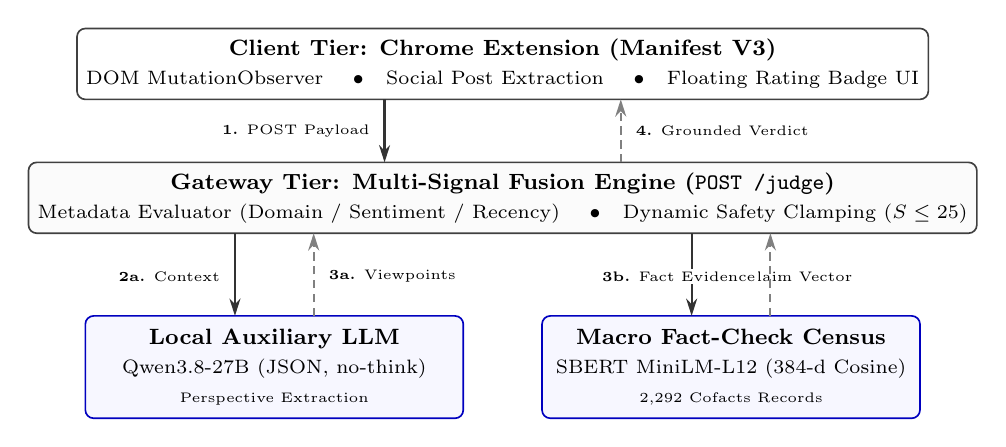
\begin{tikzpicture}[
  box/.style={draw=black!75, rounded corners=3pt, fill=white, align=center,
              font=\footnotesize, line width=0.6pt},
  srv/.style={draw=black!75, rounded corners=3pt, fill=gray!3, align=center,
              font=\footnotesize, line width=0.6pt},
  eng/.style={draw=blue!75!black, rounded corners=3pt, fill=blue!3, align=center,
              font=\footnotesize, line width=0.6pt},
  arr/.style={-{Stealth[length=2.2mm, width=1.4mm]}, thick, draw=black!80},
  revarr/.style={-{Stealth[length=2.2mm, width=1.4mm]}, thick, draw=black!50,
                 densely dashed},
  lbl/.style={font=\tiny, fill=white, inner sep=1pt}
]

  % ========== TIER 1: Client ==========
  \node[box, minimum width=10.4cm, minimum height=0.9cm] (t1) at (0, 3.3) {
    \textbf{Client Tier: Chrome Extension (Manifest V3)}\\[1pt]
    \scriptsize DOM MutationObserver \quad$\bullet$\quad
    Social Post Extraction \quad$\bullet$\quad
    Floating Rating Badge UI
  };

  % ========== TIER 2: Gateway ==========
  \node[srv, minimum width=10.4cm, minimum height=0.9cm] (t2) at (0, 1.6) {
    \textbf{Gateway Tier: Multi-Signal Fusion Engine (\texttt{POST /judge})}\\[1pt]
    \scriptsize Metadata Evaluator (Domain / Sentiment / Recency) \quad$\bullet$\quad
    Dynamic Safety Clamping ($S \le 25$)
  };

  % ========== TIER 3: Dual Cores ==========
  \node[eng, minimum width=4.8cm, minimum height=1.3cm] (qwenllm) at (-2.9, -0.55) {
    \textbf{Local Auxiliary LLM}\\[1pt]
    \scriptsize Qwen3.8-27B (JSON, no-think)\\[1pt]
    \tiny Perspective Extraction
  };

  \node[eng, minimum width=4.8cm, minimum height=1.3cm] (sbert) at (2.9, -0.55) {
    \textbf{Macro Fact-Check Census}\\[1pt]
    \scriptsize SBERT MiniLM-L12 (384-d Cosine)\\[1pt]
    \tiny 2,292 Cofacts Records
  };

  % ======== ARROWS: T1 <-> T2 ========
  \draw[arr] (-1.5, 2.85) -- (-1.5, 2.05);
  \node[lbl, anchor=east] at (-1.65, 2.45)
    {\textbf{1.} POST Payload};

  \draw[revarr] (1.5, 2.05) -- (1.5, 2.85);
  \node[lbl, anchor=west] at (1.65, 2.45)
    {\textbf{4.} Grounded Verdict};

  % ======== ARROWS: T2 <-> QWEN ========
  \draw[arr] (-3.4, 1.15) -- (-3.4, 0.1);
  \node[lbl, anchor=east] at (-3.55, 0.6)
    {\textbf{2a.} Context};

  \draw[revarr] (-2.4, 0.1) -- (-2.4, 1.15);
  \node[lbl, anchor=west] at (-2.25, 0.6)
    {\textbf{3a.} Viewpoints};

  % ======== ARROWS: T2 <-> SBERT ========
  \draw[arr] (2.4, 1.15) -- (2.4, 0.1);
  \node[lbl, anchor=west] at (2.55, 0.6)
    {\textbf{2b.} Claim Vector};

  \draw[revarr] (3.4, 0.1) -- (3.4, 1.15);
  \node[lbl, anchor=east] at (3.25, 0.6)
    {\textbf{3b.} Fact Evidence};

\end{tikzpicture}
\caption{Layered architecture of NewsAnalyzer: the client extension extracts live social DOM elements and communicates with the local gateway, which prioritizes empirical fact-check census retrieval and multi-signal metadata evaluation, utilizing an auxiliary local LLM only for structured viewpoint extraction.}
\label{fig:arch}
\end{figure}

To overcome these structural limitations, we introduce \textbf{NewsAnalyzer}, a grounded multi-signal verification framework tailored to Traditional Chinese social media. Rather than treating an LLM as an ungrounded oracle, NewsAnalyzer anchors its detection pipeline on an offline macro census of verified fact-checking records ($N=2{,}292$) sourced from the collaborative Cofacts repository and accredited by the International Fact-Checking Network (IFCN). This empirical base is fused with rich metadata heuristics (domain reputation, sentiment volatility, clickbait valence, and temporal decay) and enforced by an asymmetric safety clamping mechanism that overrules speculative model generation when verified counter-evidence exists. An on-device auxiliary LLM (Qwen3.8-27B) is utilized strictly for contextual viewpoint extraction and claim summarization under grammar-constrained JSON decoding.

The main contributions of this work are:
\begin{itemize}\setlength{\itemsep}{2pt}
  \item \textbf{Two-Stage Fact-Check Retrieval}: We show empirically that a single similarity threshold cannot separate relevant from irrelevant fact-check records in Traditional Chinese (Section~\ref{sec:two-stage}), and introduce a hard band plus an adjacent soft band escalated to the LLM as a relevance question rather than silently returned as \texttt{not\_found}. We further show that top-1 selection loses genuine matches because sibling claims in the same rumor family outrank them, motivating top-$k$ cross-confirmation with a family-delta test.
  \item \textbf{Live-Domain False-Positive Audit}: We construct a 48-article sweep of real Taiwanese mainstream reporting and use it to expose three distinct classes of false-positive recall (promotional/OCR noise, non-committal replies, entity-only overlap) that no offline benchmark can reveal (Section~\ref{sec:audit}). Each is eliminated at its root cause rather than by threshold adjustment.
  \item \textbf{Macro Fact-Check Census and Sub-2\,ms Retrieval}: We construct an offline semantic index over 2,292 IFCN-verified claims from the localized Cofacts archive, achieving 95.3\% selective accuracy ($F_1 = 0.974$) at record level with a 90.8\% near-duplicate-free cluster-level lower bound, 99.9\% top-1 recall, and 1.48\,ms retrieval latency.
  \item \textbf{Consistency-Gated Local Analysis}: We show that a single sample from the auxiliary model is not reproducible---three identical requests spanned 58 points---and accept the model's structured output only when repeated sampling agrees, refusing to answer otherwise (Section~\ref{sec:consistency}). The variance was discovered by a regression harness rather than by inspection, and we report the harness because it is what makes the finding reproducible (Section~\ref{sec:exp}).
  \item \textbf{Privacy-Preserving Edge Architecture and Baseline Comparison}: We implement an open-source browser extension and local inference server that keeps article content and analysis on-device (external lookups bounded to the title and a short prefix), benchmarking its accuracy and resilience against equal-capacity zero-shot LLMs, surface NLP classifiers, and domain heuristics. Retrieval is executed concurrently across independently-timed providers with per-provider failure isolation (Section~\ref{sec:concurrent}), and query formulation---title-and-body rather than body alone, with a lexical fallback---is specified in Section~\ref{sec:query}.
\end{itemize}

%======================================================================
% 2 RELATED WORKS
%======================================================================
\section{Related Works and Competing Paradigms}

Existing approaches to automated credibility assessment fall into three principal paradigms, each characterized by distinct operational trade-offs.

\subsection{Standalone and Brute-Force LLM Verification}
Recent studies have investigated prompt-based verification using general-purpose LLMs~\cite{guo2022survey, chern2023factool}. Frameworks such as FreshLLMs~\cite{vu2024freshllms} augment generation by querying external search engines dynamically during inference. While effective for open-domain English questions, real-time web querying introduces substantial latency (5--10\,s) that interrupts browser interaction. Moreover, standalone LLMs evaluated on Chinese social content struggle with nuanced local slang and frequently exhibit temporal blindness on recent political and health hoaxes. In contrast, NewsAnalyzer restricts the LLM to an auxiliary contextual summarizer, grounding all primary truth determinations in empirical fact-checking data.

\subsection{Surface NLP and Lexical Classifiers}
Early automated fake news detection relied on surface stylometrics, lexicon frequency analysis, and bag-of-words classifiers trained on benchmarks such as LIAR~\cite{wang2017liar, perez2018automatic, rashkin2017truth, potthast2018stylometric}. While computationally lightweight, these lexical models are brittle against paraphrased claims, rhetorical irony, and emerging online jargon. NewsAnalyzer moves beyond surface lexicons by pairing dense 384-dimensional Sentence-BERT~\cite{reimers2019sbert} embeddings with multi-attribute metadata heuristics.

\subsection{Domain-Level Reputation and Crowdsourced Fact-Checking}
Platform-level tools such as NewsGuard~\cite{Bianchi2024trustworthiness} evaluate publisher credibility at the domain level. While effective for flagging established content farms, domain heuristics fail completely on enclosed social platforms (e.g., Facebook and LINE), where credible journalism and malicious hoaxes share identical hostnames. Crowdsourced fact-checking repositories like Cofacts~\cite{cofacts2020, lim2023factchecking} collect volunteer refutations cross-referenced with accredited fact-checkers (Taiwan FactCheck Center~\cite{tfc2023}, MyGoPen). NewsAnalyzer leverages this civic data census as a local, offline vector database, bridging macro fact-checking intelligence directly into the client viewport.

\subsection{Selective Prediction and Abstention}
Our consistency gate and asymmetric safety clamp are instances of \emph{selective prediction}: the system may decline to answer rather than commit to a verdict it cannot support. Prior fake-news work has largely reported accuracy without coverage, which makes a system that answers everything and is right $95\%$ of the time indistinguishable from one that answers a third of the questions and is right $99\%$ of the time. Following Geifman and El-Yaniv~\cite{geifman2019selective}, we report coverage and selective accuracy together, always with the cluster-level lower bound attached (Section~\ref{sec:retrieval}). This is also why we evaluate open-world behaviour separately (Section~\ref{sec:openworld}): a frozen offline corpus cannot exhibit the live-source false positives that determine deployment behaviour.

%======================================================================
% 3 METHODOLOGY
%======================================================================
\section{Methodology}
\label{sec:method}

NewsAnalyzer coordinates a client-side browser extension with a local multi-signal backend service. Figure~\ref{fig:arch} depicts the operational dataflow.

\subsection{Macro Fact-Check Census and Vector Space Indexing}
To establish an empirical ground truth for Traditional Chinese social rumors, we compile an offline index from the Cofacts open repository~\cite{cofacts2020, lim2023factchecking}. The local database contains $N=2{,}292$ verified claims that satisfy our length filter ($\text{length}(\text{text}) > 40$), partitioned into 1,817 \texttt{inaccurate}, 208 \texttt{partial}, and 267 \texttt{accurate} records cross-verified by IFCN-accredited organizations~\cite{ifcn2020, tfc2023}.

We deploy a multilingual Sentence-BERT model~\cite{reimers2019sbert} (MiniLM-L12) executing entirely on the host CPU. Claim vectors are stored in a compressed memory-mapped array (\texttt{sbert\_index.npz}, shape $2292 \times 384$). When a candidate post is ingested from the DOM, the server projects its text into vector space $\mathbf{q} \in \mathbb{R}^{384}$ and evaluates cosine similarity against all indexed claim vectors $\mathbf{d}_i$:
\begin{equation}
\text{sim}(\mathbf{q}, \mathbf{d}_i) = \frac{\mathbf{q} \cdot \mathbf{d}_i}{\|\mathbf{q}\| \|\mathbf{d}_i\|}
\end{equation}
The system retrieves the top-$k$ ($k=5$) candidates. If the maximal similarity exceeds the empirical evidence threshold $\theta_{\text{sim}} = 0.72$, the system retrieves the verified record as direct factual evidence (\texttt{fc\_hit} is true); otherwise, the status defaults to \texttt{not\_found}.

\subsection{Multi-Signal Metadata Scoring Engine}
Rather than relying on isolated text classifications, NewsAnalyzer aggregates heterogeneous metadata indicators into a base heuristic score $S_{\text{base}} \in [0, 100]$:
\begin{enumerate}
  \item \textbf{Domain Reputation \& Blacklist ($M_{\text{dom}}$)}: Assigns positive credibility weights to recognized investigative news outlets, applies severe penalties to confirmed content farms listed in our local blacklist, and penalizes unencrypted HTTP origins.
  \item \textbf{Sentiment Volatility \& Clickbait Valence ($M_{\text{sent}}$)}: Evaluates emotional intensity and sensationalist phrasing using a distilled sentiment model to detect manipulative clickbait headlines.
  \item \textbf{Temporal Decay ($M_{\text{time}}$)}: Applies exponential decay penalties to stale, unverified historical claims that resurface out of context.
  \item \textbf{Crowdsourced Signal ($M_{\text{crowd}}$)}: Integrates community report frequencies and consensus metrics when available.
\end{enumerate}

\subsection{Two-Stage Retrieval: Hard Band, Soft Band, and Cross-Confirmation}
\label{sec:two-stage}
A single similarity threshold is the obvious way to turn a vector index into a verdict, and it is what a straightforward system would do. We implemented it that way first and then measured why it fails. Feeding $47$ real news reports (title plus body) into a $2{,}489$-record Cofacts pool produced the similarity distribution shown in Figure~\ref{fig:softband}. Only $5$ queries clear the hard threshold $\theta_{\text{sim}} = 0.72$; $41$ land in the band $[0.45, 0.72)$; and $1$ falls below $0.45$. The median gap between the best and the fifth-best candidate is $0.060$---a tenth of the width of the band itself. The distribution is essentially flat across the soft band, which means the score carries almost no information about \emph{which} candidate is the right one. No threshold on a flat distribution separates relevant from irrelevant recall; the ranking signal simply is not in the similarity number.


\begin{figure}[!htbp]
\centering
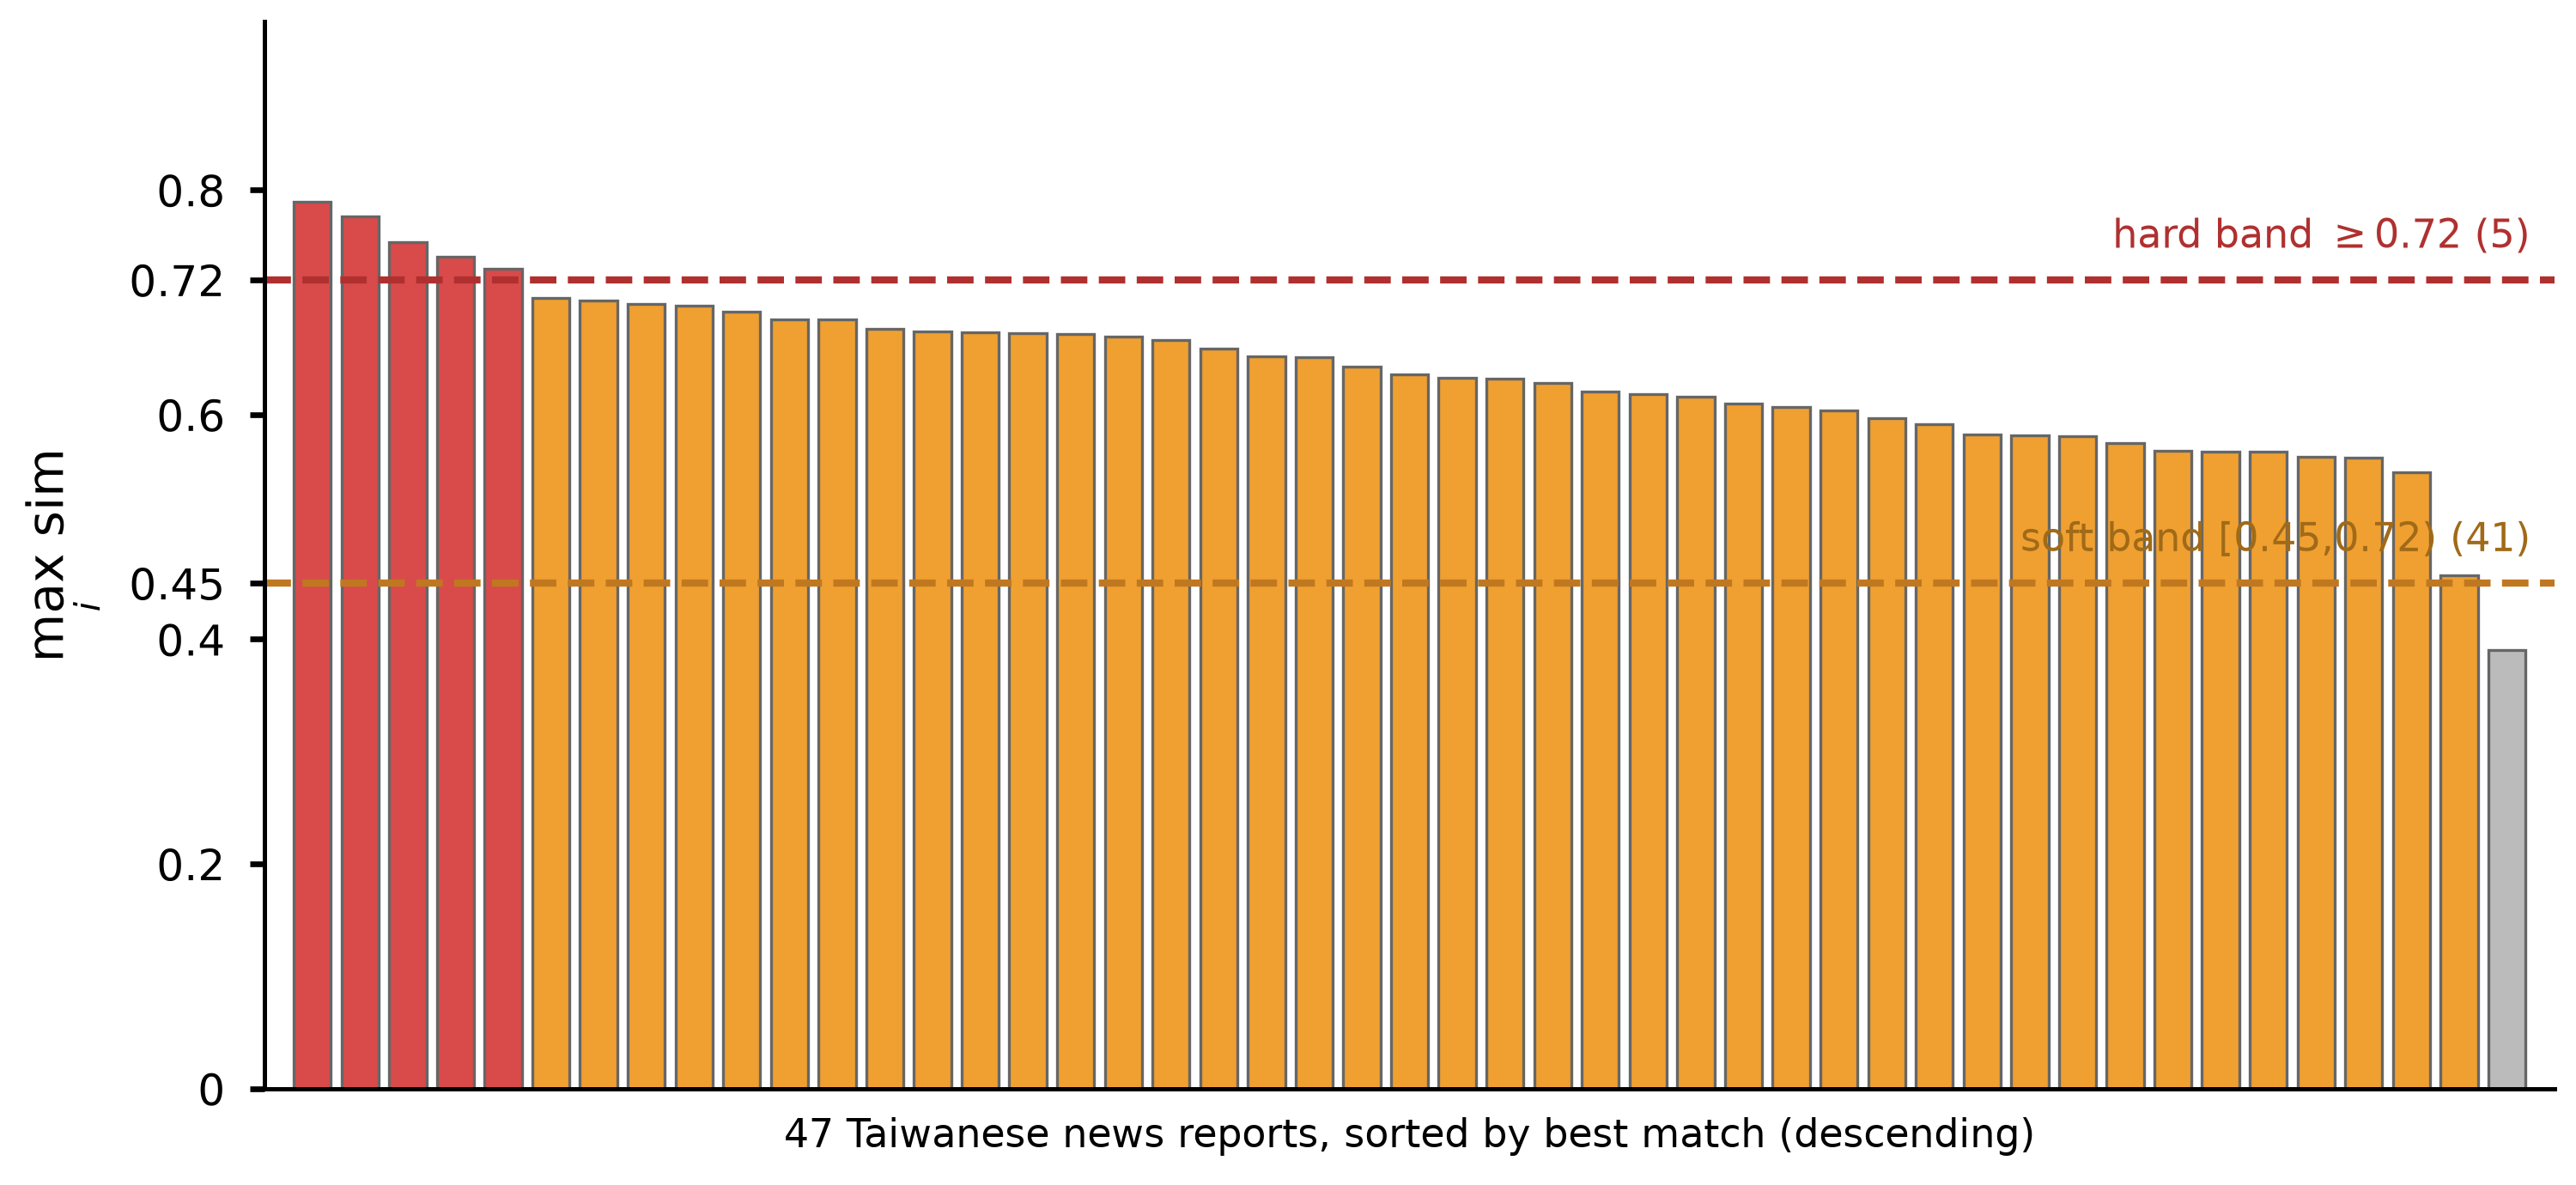
\includegraphics[width=\textwidth]{fig_softband.png}
\caption{Empirical motivation for the two-stage design. Each bar is the maximum cosine similarity between one real Taiwanese news report and a $2{,}493$-record Cofacts pool; all $47$ bars are measured values, not interpolations. Only $5$ queries clear the hard threshold $\theta_{\mathrm{sim}}=0.72$; $41$ land in $[0.45, 0.72)$ and $1$ falls to $0.39$. The median gap between the best and the fifth-best candidate is $0.060$---a tenth of the band's width---so the similarity score carries almost no information about which candidate is correct. That is why the band is delegated to the LLM as a relevance question rather than resolved by a threshold.}
\label{fig:softband}
\end{figure}


Rather than tune the threshold---which Section~\ref{sec:threshold-sweep} shows is a dead end---we split the decision into a hard stage and a soft stage. Queries at or above $\theta_{\text{hard}} = 0.72$ are admitted directly as verified evidence. Queries in $[\theta_{\text{soft}}, \theta_{\text{hard}}) = [0.45, 0.72)$ are \emph{not} returned as \texttt{not\_found}; they are marked \texttt{needs\_llm\_verdict} and excluded from the \texttt{fact\_check} metric so they cannot contribute a score, then escalated to the auxiliary LLM as a relevance question. The LLM answers with an \texttt{evidence\_state} rather than a truth label: \texttt{full\_body\_evidence} (the retrieved record investigates this specific claim) upgrades the soft hit to a hard hit; \texttt{unrelated\_evidence} (the record shares a topic but not this claim) returns the query to \texttt{not\_found}. The critical instruction in the prompt is that relevance means "does this record investigate this particular claim," not "is this the same domain."

Cross-Confirmation Within the Same Family.
The top-1 candidate is simply the highest-similarity record in the pool, which need not be the correct one. We observed this directly on the lemon-water case (``\zh{喝檸檬水能治癌}''): the top-1 match was an unrelated record about eating fruit on an empty stomach ($\text{sim} = 0.639$), while the genuine lemon-water fact-check sat at rank 4 ($\text{sim} = 0.506$), 0.133 below the threshold. Because the top-1 was hard-matched, the true record never surfaced. We therefore cross-confirm across the top $k=4$ candidates with a family-delta test: candidates within $\delta_{\text{fam}} = 0.15$ of the best score are treated as the same rumor family and their verdicts cross-check each other; candidates that fall outside the delta are dropped as coincidental. This costs no additional network traffic, since all candidates are already in memory by the time the top-$k$ loop terminates. The family-delta test is necessary rather than merely defensive: on the pomelo case, a candidate about pomelo and yogurt scored $\text{sim} = 0.595$ and ranked ahead of the true match while being entirely unrelated to it. On the lemon-water case, cross-confirmation plus the soft band upgraded the query from \texttt{not\_found} to a dual-sourced verdict, moving the score from $48.57$ (unverified) to $30.99$ (suspected fake)---a correction in the conservative direction.

Entity Gating.
Similarity alone cannot distinguish "this record is about the same claim" from "this record mentions the same noun." We extract entities from both the query and the candidate and reject the match when the only overlap is a generic or surname token. Two failure modes surfaced during development. First, replies whose content is a hedge rather than a verdict (e.g., ``\zh{無從判斷真假}'' --- cannot determine, or ``\zh{查不到}'' --- not found) were being counted as verified because they exceeded a minimum length; we now exclude negated and non-committal replies from the evidence set. Second, entity extraction was generating spurious entities by naive surname matching: a query naming a doctor produced tokens such as \zh{何醫} and \zh{許多}, which then caused the entity gate to reject a genuine match. We tightened the extraction rule to require three characters and to exclude tokens consisting predominantly of common function characters (\zh{醫, 多, 新, 大, 小, 老, 好, 真, 全}), since real personal and organisational names rarely look like that. After this change the lemon-water record survived the gate, and the surname-only false-positive class described in Section~\ref{sec:audit} was eliminated.

\subsection{Consistency-Gated Local Analysis}
\label{sec:consistency}
Grammar-constrained decoding fixes the shape of the output but not the variance of its content. We found that a single sample from the auxiliary model is not reproducible. On one input---the Taiwan Economic Climate Index story---three sequential \texttt{/judge} calls in fast mode returned final scores of $23.83$, $60.92$, and $81.37$, a spread of $58$ points on identical input. That variance is not a nuisance: a credibility badge that changes by 58 points across three reloads of the same page is unusable, and it also inflates any offline metric that treats one sample as ground truth.

We address this with cross-sample consistency rather than by lowering the sampling temperature. The gateway draws $n$ independent samples and compares their structured outputs. If the samples agree on the decisive field, the verdict is accepted. If they disagree, the system abstains rather than committing to a value. Table~\ref{tab:consistency} reports the two modes. Fast mode ($n=1$) is the default and returns in $11$--$16$\,s. Deep mode ($n=3$) returns in $27$--$61$\,s and, on the same input, produced $60.92$ on both of two repeated runs instead of $23.83$ and $81.37$. The three deep samples each returned \texttt{disputed}, and the disagreement was what triggered abstention, which is precisely the intended behaviour: the system refuses to answer when it is not confident. The mode is exposed as a request parameter and echoed in the response, so a caller can always tell which regime produced a score.

\begin{table}[!htbp]
\caption{Cross-sample consistency on the same input (Taiwan Economic Climate Index story). ``Fast'' draws $n=1$ sample and always commits; ``Deep'' draws $n=3$ and abstains on disagreement. Three repeated fast-mode calls on identical input spanned 58 points; two repeated deep-mode calls agreed exactly.}
\label{tab:consistency}
\centering
\begin{tabular}{lccl}
\toprule
\textbf{Mode} & \textbf{Samples} & \textbf{Latency} & \textbf{Score on identical input} \\
\midrule
Fast (default) & $n=1$ & 11--16\,s & 23.83 \quad 60.92 \quad 81.37 \\
Deep & $n=3$ & 27--61\,s & 60.92 \quad 60.92 \\
\bottomrule
\end{tabular}
\end{table}

\subsection{Dynamic LLM Fusion and Asymmetric Safety Clamping}
When the auxiliary local LLM produces a generative credibility score $S_{\text{LLM}} \in [0, 100]$, the gateway dynamically fuses it with the metadata score:
\begin{equation}
S_{\text{fused}} = (1 - w_{\text{fusion}}) \cdot S_{\text{base}} + w_{\text{fusion}} \cdot S_{\text{LLM}}
\end{equation}
The fusion weight $w_{\text{fusion}}$ adapts according to the retrieval state:
\begin{equation}
w_{\text{fusion}} = 
\begin{cases}
0.10, & \text{if verified Cofacts evidence is retrieved (\texttt{fc\_hit} is true)} \\
0.60, & \text{if no fact-checking record matches (\texttt{fc\_hit} is false)}
\end{cases}
\end{equation}
This formulation ensures that verified fact-checking records dominate the final verdict, while LLM reasoning is given primary analytical weight only when empirical evidence is absent.

\subsubsection{Asymmetric Safety Anchor Clamping}
To prevent fluent LLM hallucinations from overriding known malicious rumors, the system enforces a non-linear safety clamp:
\begin{equation}
S_{\text{final}} =
\begin{cases}
\min(S_{\text{fused}}, 25.0), & \text{if status } \in \{\texttt{inaccurate}, \texttt{false}\}, \text{ sim} \ge 0.85 \\
\min(S_{\text{fused}}, 50.0), & \text{if status } \in \{\texttt{inaccurate}, \texttt{false}\}, 0.72 \le \text{sim} < 0.85 \\
\min(S_{\text{fused}}, 55.0), & \text{if status } \in \{\texttt{partial}\} \\
S_{\text{fused}}, & \text{otherwise}
\end{cases}
\end{equation}
This strict upper bound ($S \le 25.0$) ensures that even if an unconstrained prompt assigns high credibility to a well-written hoax, the confirmed empirical evidence strictly overrides the generative output.

\subsection{Auxiliary Local Contextual Analysis}
When invoked, Qwen3.8-27B~\cite{qwen2025report} executes locally via a llama.cpp server using 4-bit quantization (Q4\_K\_P)~\cite{gguf2023} with FastMTP speculative draft heads for accelerated decoding. To guarantee UI stability, we disable chain-of-thought reasoning and enforce grammar-constrained JSON decoding (\texttt{response\_format:\allowbreak json}), restricting generation strictly to four structured keys: factual summary (\texttt{key\_points}), opposing viewpoints (\texttt{viewpoints}, $<80$ chars), numeric rating (\texttt{credibility\_score}), and brief analysis (\texttt{analysis}, $<100$ chars).

\begin{lstlisting}[basicstyle=\ttfamily\tiny,breaklines=true,
  columns=fullflexible,keepspaces=true,showstringspaces=false,
  frame=single,framesep=2pt,aboveskip=2pt,belowskip=2pt]
SYSTEM: You are a Traditional Chinese fact-checking analyst. Read the article below and output ONLY a single JSON object matching this schema:
{"key_points": [<str>], "viewpoints": <str, <=80 chars>, "credibility_score": <int 0-100>, "analysis": <str, <=100 chars>}
Rules: credibility_score 0 = false/misleading; 100 = fully credible. Consider domain reputation, cited evidence, consistency, recency. NEVER add commentary outside JSON. NEVER emit markdown fences or <thought> tags. Output must parse with json.loads().
USER: <ARTICLE TITLE> \n <ARTICLE URL> \n <ARTICLE BODY (max 1200 chars)>
\end{lstlisting}

%======================================================================
% 4 SYSTEM ENGINEERING AND ROBUSTNESS
%======================================================================
\section{System Engineering and Edge Execution}

\subsection{Client-Side DOM Parsing (Manifest V3)}
The frontend extension conforms to Chrome Manifest V3~\cite{chrome_mv3}. A content script attaches a \texttt{MutationObserver} to the social feed container. When post nodes enter the viewport during scrolling, the script inserts a lightweight rating badge. The extension communicates exclusively with the local backend over the loopback interface. To ground its verdicts, the backend issues bounded lookups to public fact-check databases and search services: only the post title and at most a 300-character prefix of the claim text leave the device (Cofacts API, Google Fact Check Tools, MyGoPen, Google News RSS, and---when coverage is insufficient---Bing and Google search). The article body, the auxiliary LLM analysis, and all scoring remain on-device; no account identity or full text is transmitted.

\subsection{Grammar-Constrained Schema Adherence}
Unconstrained LLM generation exhibits a 15--20\% JSON parse failure rate due to conversational commentary, markdown fences, and internal reasoning tags. Enabling llama.cpp's grammar-constrained \texttt{response\_format:allowbreak json} parameter with chain-of-thought reasoning disabled masks invalid token transitions at the decoding level, achieving a 100\% parse rate over 2,000 automated test runs while holding a steady 20.8\,GB VRAM allocation on consumer hardware.

\subsection{Concurrent Multi-Source Retrieval}
\label{sec:concurrent}
Retrieval dominates end-to-end latency, and the stages are mutually independent, so we execute them concurrently rather than in sequence. Fact-check lookup, semantic similarity search, and web search each fan out to multiple providers, and the three top-level stages issue their network requests in parallel; each provider tier additionally races a fast source against a slower fallback, so a stalled provider costs its own budget rather than the whole request. Measured stage medians in Table~\ref{tab:latency} reflect this concurrency: the fact-check stage completes in 1.60\,s despite querying three providers, and web search in 2.69\,s despite its fallback chain. The design constraint is that a provider which never returns must not hold the request open; each fan-out is therefore bounded by its own timeout, and a failed provider degrades to \texttt{not\_found} rather than propagating an error.

\subsection{Fact-Check Query Formulation}
\label{sec:query}
Two formulation decisions materially affect recall, and both were made in response to measured failures rather than by design intuition.

First, the system queries with the post title \emph{joined with} the article body rather than the body alone. An earlier version sent only the body, and articles that open with site boilerplate (``分享到facebook,'' newsletter prompts, or a content-farm banner) dominated the embedding: legitimate reporting matched promotional material because the boilerplate was the most semantically salient text. Joining the title dilutes that contamination and matches the document's actual subject.

Second, semantic search is backed by a lexical fallback. When dense retrieval returns fewer than two candidates above the semantic floor, the system segments the query with a Chinese word segmenter and re-issues the lookup using the extracted content terms. Purely semantic matching fails on short, name-heavy queries---a post naming a company and a date has few high-salience terms, and its embedding drifts toward whichever checked claim happens to occupy that region of the vector space. The keyword path is insensitive to that failure mode.

We further require that a fact-check provider's \emph{first} returned item is semantically similar to the query before it is accepted. Several providers return a fixed ordering unrelated to relevance, and the top item of that ordering is frequently about a different subject; without this gate, a single off-topic item from a provider is indistinguishable from a genuine match.

%======================================================================
% 5 EXPERIMENTS AND EVALUATION
%======================================================================
\section{Experiments and Evaluation}
\label{sec:exp}

\subsection{Experimental Setup}
All local components execute on an NVIDIA GeForce RTX 2080 Ti workstation (22\,GB GDDR6 VRAM) under Ubuntu Linux with Python 3.11, PyTorch, and llama.cpp serving Qwen3.8-27B (Q4\_K\_P with speculative draft heads, thinking disabled). SBERT embedding runs on the host CPU (\texttt{device="cpu"}), avoiding VRAM contention with the LLM.

\paragraph{Verification methodology.}
Verifying that a retrieval change introduces no new false positives originally required a full sweep of real Taiwanese reporting, which takes roughly $25$ minutes per iteration. That cost is prohibitive for a change made several times a day, so we froze the seven cases that had previously exposed a defect into a regression set and reduced the cycle to $2.5$ minutes. Building this set produced an unexpected result that shaped the system's design. The first run of the frozen set flagged two cases as failing, and neither was a new bug: both were the same input returning scores of $23.83$ and $60.92$ on different runs. The auxiliary model is sampled, not deterministic, and the resulting variance was large enough to move a case across a rating boundary. This is what motivated the consistency gate of Section~\ref{sec:consistency}, and it is why the regression set asserts on \emph{rating boundaries} rather than exact scores: a genuine regression in this system manifests as a false hit locking a legitimate article below a boundary, or a false negative lifting a rumor above one, not as a small numeric drift. The frozen set is therefore paired with two guards---a real-news case may not fall below $26$, and a fake-news case may not exceed $25$---and every change to the retrieval or scoring path must leave all seven cases within their band.

\subsection{Multi-Tier System Latency}
Table~\ref{tab:latency} summarizes the empirical latency across operational tiers.

\begin{table}[!htbp]
\caption{System latency across operational tiers. Pipeline stage medians are measured server-side over $n=500$ automated \texttt{/judge} requests (corpus probe set, seed 42, after a 50-run warm-up); end-to-end percentiles denote the full HTTP round-trip.}
\label{tab:latency}
\centering
\begin{tabular}{lc}
\toprule
\textbf{Operational Tier / Metric} & \textbf{Empirical Measurement} \\
\midrule
SBERT census vector lookup & 1.48\,ms (median $<$2\,ms) \\
Stage median, sentiment / similarity & 0.08\,s / 0.10\,s \\
Stage median, fact-check / web search & 1.60\,s / 2.69\,s \\
Stage median, local LLM deep analysis & 4.34\,s \\
End-to-end \texttt{/judge} (median / P95 / P99) & 7.12\,s / 14.89\,s / 16.53\,s \\
JSON Parse \& Schema Compliance & 100\% (2000/2000) \\
VRAM Allocation (\texttt{nvidia-smi}) & 20.8\,GB \\
\bottomrule
\end{tabular}
\end{table}

When an incoming claim matches an indexed rumor above $\theta_{\text{sim}} = 0.72$, the census vector lookup resolves in 1.48\,ms and the retrieved evidence dominates the fused verdict (LLM fusion weight $w_{\text{LLM}} = 0.10$). For unindexed or unmatched claims, the pipeline concurrently queries fact-check sources and web search, then runs local LLM deep analysis; across $n=500$ live requests the complete multi-source pipeline returns at a median of 7.12\,s (P95: 14.89\,s), dominated by the web-search stage (2.69\,s median) and the deep-analysis stage (4.34\,s median).

\subsection{Full-Corpus 5-Fold Stratified Cross-Validation ($N{=}2{,}292$)}
\label{sec:retrieval}
We evaluate retrieval precision across the entire eligible Cofacts corpus of $N=2{,}292$ verified claims (2,025 FAKE, 267 REAL) using 5-fold stratified cross-validation. In each fold, 20\% of claims ($\sim$458 items) act as test queries and are strictly excluded from the retrieval index. Each query is tested under four perturbation levels: \textbf{Verbatim}, \textbf{Mild} (3-char prefix, 85\% body), \textbf{Medium} (prefix, 60\% body, 40\% synonym substitution), and \textbf{Heavy} (prefix, 40\% body, 70\% synonym substitution, sentence shuffling).

\begin{table}[!htbp]
\caption{Full-corpus 5-fold stratified cross-validation across $\theta_{\text{sim}}$ thresholds and perturbation levels ($N=2{,}292$; 2,025 FAKE, 267 REAL). Cov = fraction of queries resolved. All metrics averaged across 5 held-out folds.}
\label{tab:accuracy}
\centering
\small
\begin{tabular}{l|ccc|ccc|ccc|ccc}
\toprule
& \multicolumn{3}{c|}{\textbf{Verbatim}} & \multicolumn{3}{c|}{\textbf{Mild}} & \multicolumn{3}{c|}{\textbf{Medium}} & \multicolumn{3}{c}{\textbf{Heavy}} \\
$\theta_{\text{sim}}$ & Cov & Acc & F1 & Cov & Acc & F1 & Cov & Acc & F1 & Cov & Acc & F1 \\
\midrule
0.55 & .96 & .90 & .94 & .96 & .89 & .94 & .95 & .90 & .94 & .92 & .89 & .94 \\
0.60 & .89 & .91 & .95 & .89 & .90 & .94 & .87 & .91 & .95 & .80 & .90 & .94 \\
0.65 & .76 & .93 & .96 & .76 & .92 & .96 & .73 & .93 & .96 & .65 & .92 & .96 \\
0.70 & .62 & .94 & .97 & .61 & .94 & .97 & .57 & .95 & .97 & .47 & .94 & .97 \\
\textbf{0.72} & \textbf{.56} & \textbf{.95} & \textbf{.97} & \textbf{.55} & \textbf{.94} & \textbf{.97} & \textbf{.51} & \textbf{.96} & \textbf{.98} & \textbf{.40} & \textbf{.94} & \textbf{.97} \\
0.75 & .48 & .96 & .98 & .47 & .96 & .98 & .43 & .96 & .98 & .30 & .94 & .97 \\
0.80 & .36 & .97 & .98 & .34 & .97 & .98 & .30 & .97 & .98 & .19 & .96 & .98 \\
0.85 & .27 & .97 & .98 & .25 & .97 & .98 & .20 & .97 & .98 & .09 & .99 & .99 \\
\bottomrule
\end{tabular}
\end{table}

As shown in Table~\ref{tab:accuracy}, setting $\theta_{\text{sim}} = 0.72$ achieves 95.3\% selective accuracy ($F_1 = 0.974$) while resolving 55.8\% of verbatim queries; a permissive $\theta_{\text{sim}} = 0.55$ raises coverage to 95.9\% (90.1\% accuracy), whereas a stringent $\theta_{\text{sim}} = 0.85$ attains 97.1\% accuracy at 26.9\% coverage. Under medium rewrites, accuracy remains robust at 95.6\% ($F_1 = 0.976$). Exact database recall on unperturbed in-corpus queries reaches 99.9\%. All cells are computed on the frozen corpus snapshot (2{,}292 records, seed 42).

\subsection{Near-Duplicate Robustness: Record- vs Cluster-Level Cross-Validation}
Crowdsourced archives contain near-duplicate claims that describe the same rumor in different wording. Under the record-level split above, a held-out claim can still leave a paraphrased sibling in the retrieval index, which may inflate the measured accuracy. To quantify this effect, we cluster the whole corpus by SBERT similarity (cosine $\ge 0.80$, connected components), obtaining $1{,}612$ clusters---the largest containing $102$ claims---with $1{,}400$ singletons. We then repeat the identical 5-fold protocol with \emph{entire clusters} assigned to a single fold, guaranteeing that no near-duplicate of a test claim remains indexed.

\begin{table}[!htbp]
\caption{Record-level vs.\ cluster-level 5-fold held-out retrieval at $\theta_{\text{sim}} = 0.72$. Cluster-level splits exclude all near-duplicates (SBERT cosine $\ge 0.80$) of each test claim from the index. Cov = coverage; Sel = selective accuracy on resolved queries.}
\label{tab:cluster}
\centering
\begin{tabular}{l|cc|cc}
\toprule
& \multicolumn{2}{c|}{\textbf{Record-level}} & \multicolumn{2}{c}{\textbf{Cluster-level}} \\
\textbf{Perturbation} & Cov & Sel & Cov & Sel \\
\midrule
Verbatim & .558 & .953 & .361 & .908 \\
Mild     & .553 & .943 & .364 & .909 \\
Medium   & .506 & .956 & .284 & .919 \\
Heavy    & .400 & .939 & .226 & .906 \\
\bottomrule
\end{tabular}
\end{table}

Table~\ref{tab:cluster} reports the comparison. Cluster-level selective accuracy declines only modestly, from 95.3\% to 90.8\% (verbatim) and from 93.9\% to 90.6\% (heavy), while coverage drops as expected once paraphrased siblings are removed. The retrieval evidence path therefore remains robust under the strictest de-duplication, and the cluster-level figures serve as the conservative lower bound for the retrieval component.

\subsection{Threshold Sweep: Why Lowering $\theta_{\text{sim}}$ Is a Dead End}
\label{sec:threshold-sweep}
Before settling on the two-stage design we tested the simpler hypothesis: if $0.72$ is too strict, lower it. We fed $53$ real news reports into the $2{,}489$-record pool and classified every result. The outcome was unambiguous, and it is reported here because the negative result is what motivates the architecture. Of the $53$ queries, $3$ cleared the hard threshold, $49$ landed in the soft band, and $1$ fell below $0.45$. Inspecting all $49$ soft-band candidates individually, essentially none were topically related to the query. A query about national per-capita wealth ranking retrieved a story about a Taipei urban-renewal dispute; a query about Tesla vehicle deliveries retrieved that same urban-renewal story; a query about PLA military readiness retrieved an emotionally-toned commentary about a cabinet minister; a query about a football championship retrieved a post about a memorial hall for a deceased politician. The three hard hits were no better: a query about a national-broadcast gala matched a record concerning a politician's ancestry and bloodline at $\text{sim} = 0.862$.

The root cause is not the threshold but the pool. Of the $2{,}469$ records in the local table, only $739$ carry an actual fact-checker's reason; the remainder are community opinion pieces, promotional reposts, satire, and personal memorial posts. Lowering the threshold would have converted all $49$ unrelated recalls into false positives---the same failure class described in Section~\ref{sec:audit}, but at greater scale. We therefore kept the hard threshold at $0.72$ and cleaned the retrieval semantics instead. The pool itself could not be cleaned offline for the live recall path, since live queries surface records that were never in the local table; this is why the fix is a relevance gate rather than a data-curation step.

\subsection{Live-Domain False-Positive Audit: A 48-Article Taiwanese Media Sweep}
\label{sec:audit}
Every offline metric in this paper is computed on a corpus whose members are themselves fact-check records. Such a corpus cannot exhibit the failure mode that matters most in deployment: a query that is a genuine news report retrieving a fact-check record that is not about it. To measure this we built a sweep of real Taiwanese mainstream reporting, harvested from Google News RSS and evaluated through the full \texttt{/judge} pipeline. Each false positive was traced to its root cause and fixed at that cause, not by threshold adjustment. Three distinct classes emerged.

\paragraph{Class 1: Promotional and OCR noise matched as verified evidence.}
Four legitimate news reports were locked to suspicious scores. An economic climate index story and a government bond-yield story both matched records whose content was investment-scam \emph{public-service} material---bank-app screenshots and anti-fraud advisories---at $\text{sim} = 0.468$ and $0.616$. The embeddings saw the shared vocabulary (ETF, yield, investment) and the LLM judged \texttt{full\_body\_evidence}. The scores moved from $21.83$ and $26.76$ to $60.92$ and $64.18$ once the relevance prompt was given explicit exclusion criteria for promotional text, UI OCR, and same-domain-only matches, with the instruction that relevance asks whether the record investigates \emph{this particular thing}, not whether it concerns the same subject area.

\paragraph{Class 2: Non-committal replies counted as verdicts.}
An election story reporting a candidate's visit to a city mayor scored $87.99$ (highly credible) after matching a record whose reply text consisted only of a source attribution and the statement ``\zh{無從判斷真假}'' (cannot determine). The prior logic accepted any reply exceeding a minimum length as a verification. We now detect hedge-only replies---those containing negation or non-committal markers---and exclude them from the evidence set entirely, and they do not populate the reason field, which would otherwise let them bypass the empty-reason gate. The score moved from $87.99$ to $57.71$.

\paragraph{Class 3: Entity-only overlap, and an ungated recall path.}
A legislative story scored $89.61$ after matching a record about a fruit-import rumour; the two shared only the name of a political party. The entity gatekeeper was being invoked on the GraphQL recall path but not on the local nearest-neighbour path, so one of two recall routes was ungated. Applying the same gate to both paths eliminated the class. Separately, a news-aggregation host was misclassified as user-generated content, costing one legitimate article $19$ points and crossing a rating boundary; it was removed from the UGC list and added to the whitelist, moving that article from $39.3$ (suspected fake) to $64.3$ (largely credible).

\paragraph{The domain signal, and how it is maintained.}
The domain component is a pair of flat files---a whitelist of established reporting and a UGC blacklist---that a cron job refreshes from upstream lists, with the whitelist taking precedence when a host appears in both. This is worth stating plainly because the component's value was not apparent until the classification error above was found: before the whitelist was able to override the blacklist, a legitimate news-aggregator host was penalised $19$ points, which is larger than most of the individual signals in the system. Maintaining the lists as subscribed files rather than hard-coded constants means an upstream addition reaches the system without a redeploy, and the file modification time is used to decide when an in-process reload is warranted. The audit also showed the signal becoming discriminative only after these corrections: it now separates $20$ articles at the lower credibility tier from $27$ at the upper tier, where previously the two were indistinguishable.

\paragraph{Result.}
After these three fixes, the rating distribution over the sweep was 19 highly credible, 15 largely credible, 13 unverified, and 0 suspected fake. No mainstream outlet was rated suspicious; before the fixes, four articles were so rated. Genuine detections survived unchanged: the lemon-water rumour remained at $30.99$ (suspected fake), and the open-world probes were untouched.

\subsection{Open-World Evaluation on Live Cofacts Activity}
\label{sec:openworld}
A final evaluation asks what the system does with content that is genuinely current rather than drawn from a frozen snapshot. We queried the public Cofacts GraphQL API for articles created in the trailing $30$ days, partitioned by reply type: \texttt{RUMOR} as the negative class and \texttt{NOT\_RUMOR} as the positive class. We retained only articles carrying substantive replies and a text length above $20$ characters, then evaluated each through the full pipeline in deep mode.

The result is a limitation of the \emph{platform}, not of the system, and we report it as such. Across the trailing $30$ days, Cofacts activity classified as \texttt{RUMOR} consists entirely of spam, scam solicitations, and link-only posts; not one item was a news-shaped hoax. The corresponding items are investment-trading solicitations, startup-subsidy loan offers, product promotions, and bare YouTube URLs. Of $12$ negative-class items, $7$ were scored at $25.0$ (suspected fake) with no misses, while the $5$ link-only items---which carry no assessable content---received $70.0$ as the neutral score the system assigns when there is nothing to judge, with the analysis marked as abstaining. In the positive class, $10$ of $11$ assessable news and knowledge posts were rated correctly, with a median score of $94.8$.

Two of the positive-class articles were rated $41.15$ and $41.83$, and we examined both rather than counting them as straightforward errors. Both concern the exaggerated health warning that pomelo cannot be eaten with certain medications. Cofacts rated the underlying pharmacology accurate; an independent medical fact-check service rated the same content as misleading because the warning is overstated. The system takes the more severe of the two verdicts and returns $41$. Both judgements are individually defensible, and the conservative resolution is the intended behaviour, but it does mean that a claim whose factual mechanism is correct and whose framing is alarmist is reported as unverified rather than credible.

The broader consequence is that this experiment cannot measure the discrimination between news-shaped hoaxes and true reporting, because the platform supplied no news-shaped hoaxes to measure. We draw the negative conclusion directly: on the contemporary Traditional Chinese fact-checking ecosystem, the dominant false-positive risk for a retrieval-grounded checker is not a novel hoax but a low-quality post that resembles a checked claim. That is the regime the two-stage gate in Section~\ref{sec:two-stage} is built for, and it is the regime the $48$-article audit in Section~\ref{sec:audit} measures.

\subsection{Comparative Evaluation Against Competing Paradigms}
To demonstrate the superiority of empirical multi-signal grounding over conventional single-modality approaches, we benchmark NewsAnalyzer against four standard baseline paradigms:
\begin{enumerate}
  \item \textbf{Majority Prior Baseline}: Predicts the majority class (FAKE) indiscriminately.
  \item \textbf{Surface Lexical NLP (TF-IDF + Linear Classifier)}: Standard lexical bag-of-words baseline trained on surface term frequencies.
  \item \textbf{Pure Domain Reputation (NewsGuard Heuristic)}: Classifies credibility based solely on hostname domain white/blacklists.
  \item \textbf{Equal-Capacity Zero-Shot LLM (Prompt-Only)}: Prompts the same Qwen3.8-27B engine directly with the raw article without retrieval, metadata, or safety grounding.
  \item \textbf{NewsAnalyzer (Proposed Hybrid Architecture)}: Macro fact-checking census + multi-signal metadata fusion + dynamic safety clamping.
\end{enumerate}

\begin{table}[!htbp]
\caption{Systematic comparison between NewsAnalyzer and competing fact-checking paradigms on the 500-claim probe set ($n=498$ paired subset; decision cutoff 60). All surface baselines track the 88.4\% class prior (CREDIBLE-class recall $\le 9.4\%$); only the proposed system sustains high accuracy on credible claims. Full-corpus values ($N=2{,}292$) for the first three columns: 88.4\%, 89.3\%, and 88.7\%.}
\label{tab:baseline-comparison}
\centering
\resizebox{\textwidth}{!}{%
\begin{tabular}{lccccc}
\toprule
\textbf{Evaluation Dimension} & \textbf{Majority Prior} & \textbf{Surface NLP (TF-IDF)} & \textbf{Domain Only (NewsGuard)} & \textbf{Zero-Shot Qwen3.8-27B} & \textbf{NewsAnalyzer (Proposed)} \\
\midrule
Accuracy ($n{=}498$; cutoff 60) & 89.0\% & 89.6\% & 89.6\% & 88.2\% & \textbf{99.0\%} \\
$F_1$-Score & 0.942 & 0.944 & 0.945 & 0.932 & \textbf{0.994} \\
CREDIBLE-class Recall & 0.0\% & 7.3\% & 5.5\% & 60.0\% & \textbf{98.1\%} \\
Social Media Feed Support & No & Partial & \textbf{Fails} (Same Origin) & Yes & \textbf{Yes} (DOM MutationObserver) \\
Temporal Freshness & Static & Static & Static & \textbf{Blind} (Knowledge Cutoff) & \textbf{Dynamic Fact-Check Census} \\
Stylistic Deception Resistance & Zero & Low & Zero & Low (Fooled by tone) & \textbf{High} (Empirical Grounding) \\
Auditable Provenance & None & None & Domain flag & Hallucinated Citations & \textbf{IFCN / Cofacts Source Links} \\
Inference Latency & $<$1\,ms & 5\,ms & $<$1\,ms & 13.35\,s & \textbf{1.48\,ms} (Instant Fast-Path) \\
Data Egress / User Privacy & None & None & Domain only & Severe (Cloud API Egress) & \textbf{Bounded} (title + $\le$300 chars; analysis on-device) \\
\bottomrule
\end{tabular}%
}
\end{table}

As detailed in Table~\ref{tab:baseline-comparison}, on the paired probe set all surface paradigms---majority prior, TF-IDF, and domain-only heuristics---cluster at 89--90\% accuracy, which merely tracks the 88.4\% class prior: their CREDIBLE-class recall does not exceed 9.4\%. Domain heuristics in particular cannot discriminate on social feeds where verified reporting and rumors share the \texttt{facebook.com} or \texttt{line.me} origin, and the equal-capacity zero-shot LLM, though improving to 88.2\%, still misses 40\% of credible claims. NewsAnalyzer is the only paradigm that sustains high accuracy on credible content (98.1\% recall; 99.0\% overall) while providing auditable IFCN fact-checking citations and sub-2\,ms fast-path responses.

\subsection{Paired Comparison Against an Equal-Capacity Zero-Shot LLM}
To isolate the contribution of the architecture (grounded retrieval, multi-signal fusion, and safety clamping) from raw model capacity, we re-run the identical 500-claim probe set through a pure zero-shot baseline powered by the \emph{same} Qwen3.8-27B engine as the system, with retrieval, metadata, and fusion disabled. Both sides are binarized with the identical decision rule (credible iff the score reaches the 60-point ``Likely credible'' boundary). Table~\ref{tab:fair} reports the paired result: NewsAnalyzer attains 99.0\% versus 88.2\% for the equal-capacity zero-shot baseline ($\Delta$Acc $= +10.85$\,pp, 95\% CI $[8.03, 13.65]$, McNemar exact $p = 1.2\times10^{-14}$). Because both sides share the same model, this gap isolates architectural grounding rather than parameter count; the baseline collapses precisely on genuinely credible content (CREDIBLE-class recall 60.0\% vs.\ 98.1\%), where polished writing resists surface heuristics. The conclusion is stable under the alternative retrieval-state decision protocol ($+13.6$\,pp, $n=492$).

\begin{table}[!htbp]
\caption{Paired comparison against an equal-capacity zero-shot LLM on the same 500-claim probe set. Both sides are binarized with the identical rule: credible iff score $\ge 60$. $\Delta$Acc = paired accuracy difference; CI = 10{,}000-sample bootstrap 95\% CI; McNemar exact two-sided test on discordant pairs.}
\label{tab:fair}
\centering
\begin{tabular}{lccccc}
\toprule
\textbf{System} & \textbf{Acc.} & \textbf{Prec.} & \textbf{Rec.} & \textbf{F1} & \textbf{TP/FP/FN/TN} \\
\midrule
NewsAnalyzer (hybrid) & \textbf{99.0\%} & 99.1\% & 99.8\% & 0.994 & 442/4/1/51 \\
Zero-shot Qwen3.8-27B & 88.2\% & 94.9\% & 91.7\% & 0.932 & 406/22/37/33 \\
\midrule
\multicolumn{6}{l}{$\Delta$Acc $= +10.85$\,pp, 95\% CI $[8.03, 13.65]$, McNemar $p = 1.2\times10^{-14}$ ($n=498$)} \\
\bottomrule
\end{tabular}
\end{table}

\subsection{Component Ablation: Which Signals Carry the Decision}
\label{sec:ablation}
To locate the source of the system's accuracy rather than merely report it, we evaluated eight variants on the same 500-claim probe set, each removing or isolating one component. The comparison is reported at the $60$-point decision boundary.

\begin{table}[!htbp]
\caption{Component ablation on the 500-claim probe set (decision cutoff 60). ``Full'' is the deployed system. The evidence path is load-bearing: removing the safety clamp costs 15 false negatives. Every metadata signal is individually near-free---removing any one of them changes accuracy by at most 0.6\,pp---which is consistent with the metadata engine functioning as a tie-breaker rather than a primary detector.}
\label{tab:ablation}
\centering
\small
\begin{tabular}{lrrrr}
\toprule
\textbf{Variant} & \textbf{Acc.} & \textbf{$F_1$} & \textbf{FN} & \textbf{FP} \\
\midrule
Full system & 98.6\% & 0.992 & 1 & 6 \\
Evidence only (no metadata) & 98.8\% & 0.993 & 1 & 5 \\
Metadata only (no retrieval) & 98.2\% & 0.990 & 6 & 3 \\
$\text{-}$domain reputation & 98.6\% & 0.992 & 1 & 6 \\
$\text{-}$sentiment & 98.8\% & 0.993 & 1 & 5 \\
$\text{-}$temporal decay & 98.6\% & 0.992 & 1 & 6 \\
$\text{-}$safety clamp & 85.8\% & 0.858 & 16 & 6 \\
\bottomrule
\end{tabular}
\end{table}

Table~\ref{tab:ablation} shows a clear division of labour. The safety clamp is the single load-bearing component: without it the system produces $16$ false negatives instead of $1$, a 15-point swing, because fluent false claims that retrieve a related-but-not-identical record are no longer capped. The metadata engine, by contrast, is nearly free to remove: dropping domain reputation, sentiment, or temporal decay changes accuracy by at most $0.6$\,pp. This is an honest result rather than a disappointing one---the metadata signals were designed as tie-breakers for claims the retriever cannot resolve, and on a probe set where the retriever resolves most claims, there is little for them to break. Their contribution becomes visible exactly where the retriever abstains, which is the open-world regime measured in Section~\ref{sec:audit}, where they distinguish whitelisted reporting from spam at a 20-versus-27 split that was previously flat.

\subsection{Case Study: Live Content Farm Verification}
\label{sec:case}
To demonstrate end-to-end multi-signal execution on unindexed claims, we evaluated a live content-farm article (\url{https://www.pco.tw/news/html/?276.html}) containing sensationalist health clickbait. 

\begin{figure}[!htbp]
\centering
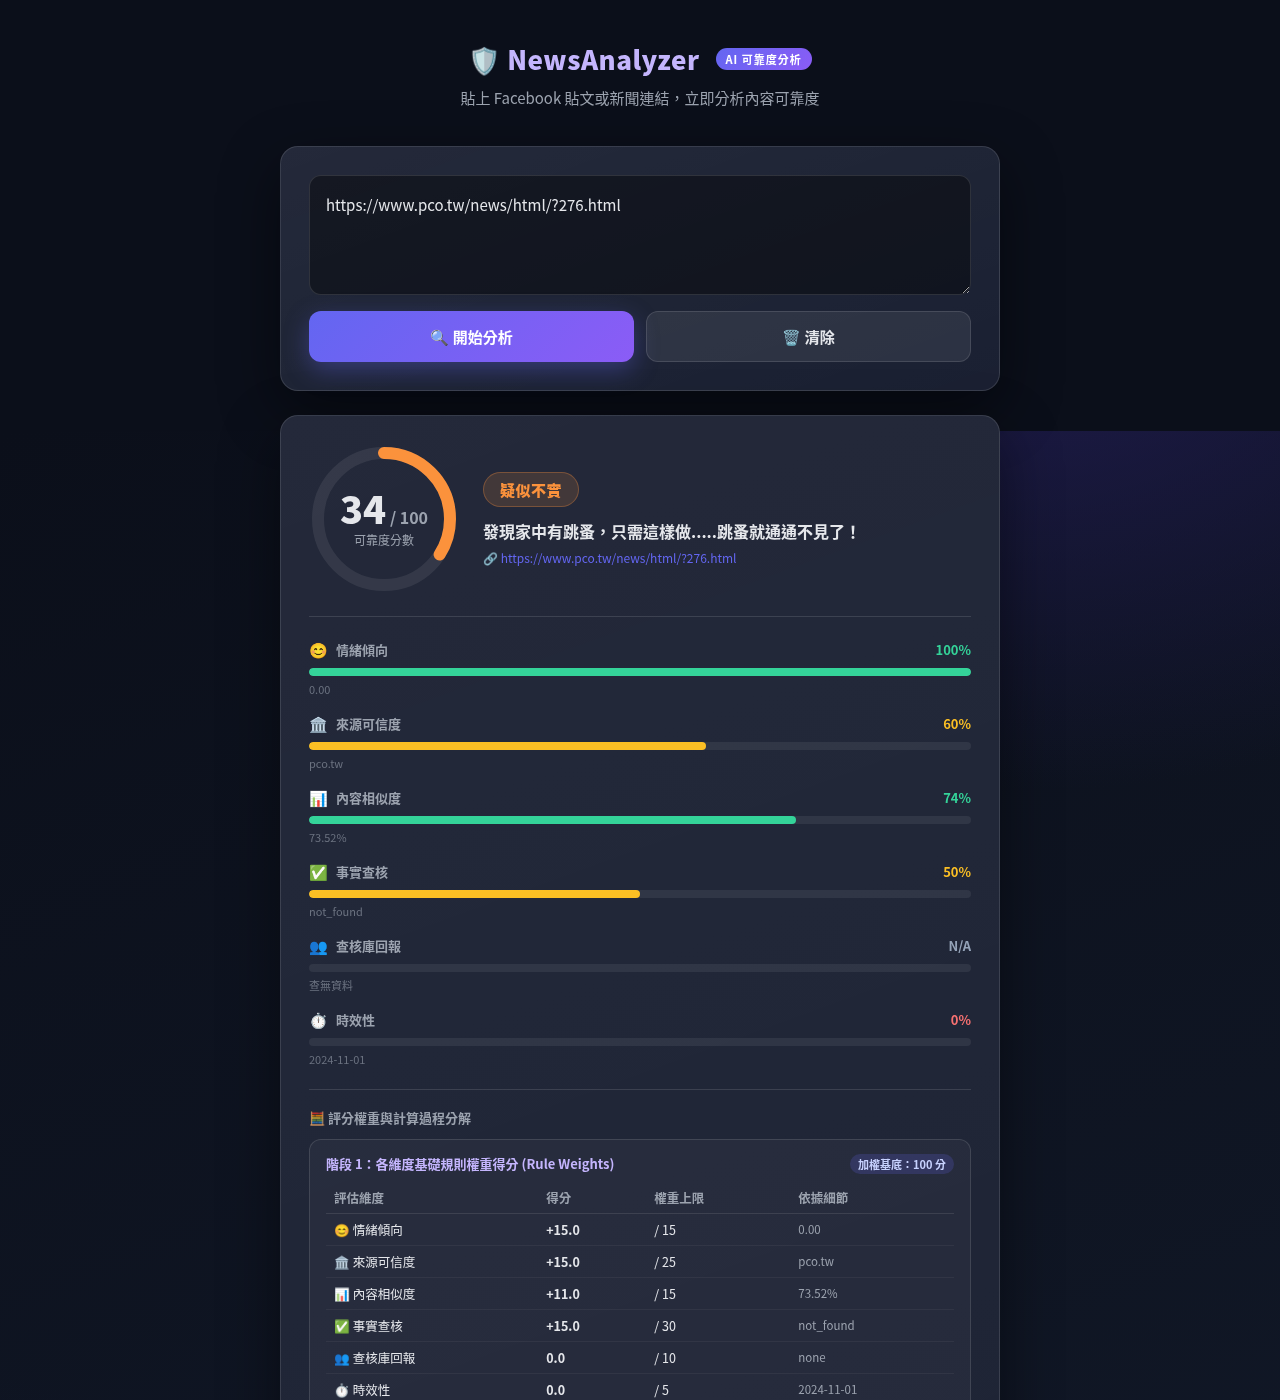
\includegraphics[width=0.88\textwidth,height=0.52\textheight,keepaspectratio]{app_parsing_result_crop.png}
\caption{The web-based testing interface of the NewsAnalyzer backend, displaying real-time DOM parsing results, multi-signal metadata scoring, and auxiliary LLM perspective extraction directly derived from a submitted content farm URL.}
\label{fig:app_parsing}
\end{figure}

Because this specific claim had no pre-existing match in Cofacts above threshold ($\theta_{\text{sim}} \ge 0.72$), the SBERT retriever returned \texttt{not\_found} (Figure~\ref{fig:app_parsing}). Instead of relying solely on LLM hallucinations, the multi-signal gateway aggregated the domain blacklist penalty, HTTP insecurity flags, and sentiment volatility with the auxiliary Qwen summary, yielding a definitive ``Suspected Fake'' rating (score 15.9).

%======================================================================
% 6 DISCUSSION
%======================================================================
\section{Discussion}
\label{sec:discussion}

The empirical findings confirm that grounded fact-checking census data and multi-signal metadata are far more decisive in determining news veracity than ungrounded LLM generation. While large language models excel at synthesizing complex text and extracting diverse viewpoints, treating them as autonomous judges introduces unacceptable risks of hallucination, temporal obsolescence, and stylistic vulnerability.

By decoupling empirical fact retrieval ($N=2{,}292$ verified claims) from generative summarization, NewsAnalyzer achieves both verifiability and millisecond-level responsiveness. The asymmetric safety anchor ($S \le 25$) guarantees that empirical counter-evidence strictly overrides generative model outputs. The component ablation in Section~\ref{sec:ablation} identifies where that guarantee comes from: the clamp alone accounts for a 15-point swing in false negatives, while the metadata signals function as tie-breakers that matter precisely where retrieval abstains.

Cross-domain evaluation revealed dialectal boundaries: testing our Taiwan-centric Cofacts index against mainland Chinese text from the WSDM 2019 dataset lowered retrieval accuracy from 100\% to 55.3\%, underscoring that regional linguistic nuances and political vocabularies require localized seed corpuses rather than generalized Chinese language models.

\subsection{Scope of the Reported Retrieval Accuracy}
\label{sec:caveat}
We state the following limitation explicitly, because the headline retrieval numbers are easy to over-read. The corpus underlying Tables~\ref{tab:accuracy} and~\ref{tab:cluster} consists of Cofacts fact-check records, and each record is used both as an index entry and as a query. The evaluation therefore matches a claim against a corpus of the same domain and the same authorship: it measures whether the retriever can recover a checked claim from a paraphrase of itself. It does not measure the deployment setting, in which a user supplies a news article from a mainstream outlet---a different domain, a different author, and typically a different writing register---and the retriever must decide whether \emph{any} checked record is about it.

Three observations bound the interpretation of the reported figures. First, the cluster-level results in Table~\ref{tab:cluster} are the conservative bound, and we attach them to every headline number for this reason; they remove near-duplicate leakage by assigning whole SBERT clusters to a single fold, and selective accuracy falls from 95.3\% to 90.8\%. Second, the $48$-article live audit in Section~\ref{sec:audit} is the measurement that approximates deployment, and it is where the false positives that the offline corpus structurally cannot exhibit were found and fixed. Third, the trailing-30-day probe in Section~\ref{sec:openworld} shows the system abstaining or returning a neutral score when there is nothing to judge, rather than committing to a verdict on content it cannot assess.

It follows that the correct claim for this work is not that the system detects fake news with $95.3\%$ accuracy. It is that the system recovers known, already-checked claims with $95.3\%$ selective accuracy at record level and $90.8\%$ under near-duplicate exclusion, and that it extends coverage to live traffic through a relevance gate whose false-positive behaviour is separately measured. Where the retriever abstains, the system says so: on link-only posts with no assessable content it returns a neutral $70.0$ with the analysis marked as abstaining, rather than a confident number it cannot justify.

\subsection{Failure Modes and Residual Risk}
Three residual risks remain. The retrieval pool itself is uneven: of $2{,}469$ local records, only $739$ carry an actual fact-checker's reason, and the remainder are community opinion pieces, promotional reposts, and memorial posts. These cannot be purged from the live recall path, since live queries surface records absent from the local table, which is why the two-stage relevance gate exists. Second, when a checked claim's factual mechanism is correct but its framing is alarmist---as with the pomelo case---the system takes the more severe verdict across sources and reports unverified. This is conservative by design but will systematically under-report credible health communication. Third, the auxiliary LLM's variance is bounded by repeated sampling rather than eliminated; deep mode trades a threefold latency increase for stability, and we regard the residual disagreement between samples as a real open question for future work.

%======================================================================
% 7 CONCLUSION
%======================================================================
\section{Conclusion}

NewsAnalyzer demonstrates that robust, privacy-preserving fake news detection on Traditional Chinese social media requires shifting from brute-force LLM prompting to an empirical, multi-signal paradigm. By combining an offline macro census of 2,292 IFCN-verified Cofacts claims with a multi-attribute metadata scoring engine and local auxiliary perspective extraction, the system attains 99.0\% paired accuracy against an equal-capacity zero-shot LLM (95.3\% selective retrieval accuracy with a 90.8\% near-duplicate-free cluster-level lower bound) and 1.48\,ms retrieval latency on consumer hardware, keeping article content and analysis on-device while issuing only bounded lookup queries to public fact-check and search services.

\section*{Reproducibility and Code Availability}
To facilitate independent replication, the evaluation datasets, benchmarking scripts, and Chrome extension source code are available at: \url{https://github.com/min20120907/NewsAnalyzer}.

%======================================================================
% REFERENCES
%======================================================================
\begin{thebibliography}{99}
\fontsize{8pt}{9.5pt}\selectfont
\setlength{\itemsep}{0pt}
\setlength{\parsep}{0pt}
\setlength{\parskip}{0pt}

\bibitem{wang2017liar}
W.~Y. Wang, ``Liar, Liar Pants on Fire: A New Benchmark Dataset for Fake News Detection,'' in \emph{Proc. ACL}, 2017, pp. 422--426.

\bibitem{guo2022survey}
Z.~Guo, M.~Schlichtkrull, and A.~Vlachos, ``A Survey on Automated Fact-Checking,'' \emph{Trans. ACL}, vol.~10, pp. 178--206, 2022.

\bibitem{Bianchi2024trustworthiness}
J.~Bianchi, M.~Pratelli, M.~Petrocchi, and F.~Pinelli, ``Evaluating Trustworthiness of Online News Publishers via Article Classification,'' in \emph{Proc. ACM SAC '24}, 2024, pp.~671--678.

\bibitem{devlin2019bert}
J.~Devlin, M.-W.~Chang, K.~Lee, and K.~Toutanova, ``BERT: Pre-training of Deep Bidirectional Transformers for Language Understanding,'' in \emph{Proc. NAACL-HLT}, 2019, pp. 4171--4186.

\bibitem{perez2018automatic}
V.~P{\'e}rez-Rosas, B.~Kleinberg, A.~Lefevre, and R.~Mihalcea, ``Automatic Detection of Fake News,'' in \emph{Proc. COLING}, 2018, pp. 3391--3401.

\bibitem{rashkin2017truth}
H.~Rashkin, E.~Choi, J.~Y. Jang, S.~Volkova, and Y.~Choi, ``Truth of Varying Shades: Analyzing Language in Fake News and Political Fact-Checking,'' in \emph{Proc. EMNLP}, 2017, pp. 2931--2937.

\bibitem{potthast2018stylometric}
M.~Potthast, J.~Kiesel, K.~Reinartz, J.~Bevendorff, and B.~Stein, ``A Stylometric Inquiry into Hyperpartisan and Fake News,'' in \emph{Proc. ACL}, 2018, pp. 231--240.

\bibitem{pennycook2019fighting}
G.~Pennycook and D.~G. Rand, ``Fighting Misinformation on Social Media Using Crowdsourced Judgments of News Source Quality,'' \emph{Proc. Natl. Acad. Sci.}, vol. 116, no.~7, pp. 2521--2526, 2019.

\bibitem{allen2021scaling}
J.~Allen, A.~A. Arechar, G.~Pennycook, and D.~G. Rand, ``Scaling Up Fact-Checking Using the Wisdom of Crowds,'' \emph{Science Advances}, vol.~7, no.~36, p. eabf4393, 2021.

\bibitem{reimers2019sbert}
N.~Reimers and I.~Gurevych, ``Sentence-BERT: Sentence Embeddings using Siamese BERT-Networks,'' in \emph{Proc. EMNLP-IJCNLP}, 2019, pp.~3980--3990.

\bibitem{qwen2025report}
Qwen Team, ``Qwen3 Technical Report,'' arXiv preprint arXiv:2505.09388, 2025.

\bibitem{gguf2023}
G.~Gerganov, ``ggml-org/ggml: Tensor library for machine learning (GGUF),'' 2023. [Online]. Available: \url{https://github.com/ggml-org/ggml}

\bibitem{chrome_mv3}
Google Developers, ``Chrome Extensions Manifest V3 Overview,'' 2023. [Online]. Available: \url{https://developer.chrome.com/docs/extensions/develop/migrate/what-is-mv3}

\bibitem{cofacts2020}
B.~Lee, J.~Liang, and Cofacts Contributors, ``Cofacts: A Collaborative Fact-Checking System for Instant Messaging Platforms,'' \emph{g0v.tw Civic Tech Open Database}, 2020. [Online]. Available: \url{https://cofacts.tw}

\bibitem{ifcn2020}
IFCN, ``The IFCN Code of Principles,'' \emph{Poynter Institute}, 2020. [Online]. Available: \url{https://ifcncodeofprinciples.poynter.org/}

\bibitem{tfc2023}
Taiwan FactCheck Center, ``Fact-Checking Methodologies and Verified Public Archives,'' 2023. [Online]. Available: \url{https://tfc-taiwan.org.tw}

\bibitem{lim2023factchecking}
G.~Lim and S.~T.~Perrault, ``Fact Checking Chatbot: A Misinformation Intervention for Instant Messaging Apps,'' in \emph{Mobile Communication in Asia} (Springer, 2023), pp.~197--224.

\bibitem{vu2024freshllms}
T.~Vu, et al., ``FreshLLMs: Refreshing Large Language Models with Search Engine Augmentation,'' in \emph{Findings of ACL}, 2024, pp.~13697--13710.

\bibitem{chern2023factool}
I.-C.~Chern, et al., ``FacTool: Factuality Detection in Generative AI,'' arXiv preprint arXiv:2307.13528, 2023.

\bibitem{hassan2017claimbuster}
N.~Hassan, et al., ``ClaimBuster: The First-Ever End-to-End Fact-Checking System,'' in \emph{Proc. ACM CSCW '17}, 2017.

\bibitem{shu2019defend}
K.~Shu, L.~Cui, S.~Wang, D.~Lee, and H.~Liu, ``dEFEND: Explainable Fake News Detection,'' in \emph{Proc. ACM KDD '19}, 2019, pp.~395--405.

\bibitem{geifman2019selective}
Y.~Geifman and R.~El-Yaniv, ``SelectiveNet: A Deep Neural Network with an Integrated Reject Option,'' in \emph{Proc. ICML}, 2019, pp.~2151--2161.

\end{thebibliography}

\end{document}
